\subsection{Proximal Gradient Descent (PGD)}\label{ssec:pgd}

In this section, we describe the PGD method, or ISTA,
to solve the block update~(\ref{eq:bcd:block-update}).
The progression is similar to that of~\citet{sls:2016}.
Define
\begin{align*}
    f(\beta)
    &=
    \frac{1}{2} \beta^\top D \beta
    - v^\top \beta
\end{align*}
as the convex (Gaussian) loss function in~(\ref{eq:bcd:block-update}).
ISTA has guaranteed convergence so long as the step-size is chosen properly.
Indeed, any step-size $\nu$ can be chosen such that
$\nu \leq \frac{1}{L}$ where $L$ is the Lipschitz constant for $\nabla f$.
Since 
\begin{align}
    \nabla f(\beta)
    &=
    D \beta - v
    \label{eq:pgd:nablaf}
    \\\implies
    \norm{
        \nabla f(\beta)
        - \nabla f(\tilde{\beta})
    }_2
    &=
    \norm{D (\beta - \tilde{\beta})}_2
    \leq
    \opnorm{D} \norm{\beta-\tilde{\beta}}_2
    \nonumber
\end{align}
we have $L \equiv \opnorm{D} \equiv \lambda_{\max}(D)$ as the largest eigenvalue of $D$.
In particular, since $D$ is diagonal, $L \equiv \max\limits_{i} D_{ii}$.

The ISTA procedure is given in Algorithm~\ref{alg:pgd:ista}.
By applying a standard Nesterov acceleration~\citep{beck:2009}, 
we have the FISTA procedure. % given in Algorithm~\ref{alg:pgd:fista}.
Additionally, we may perform adaptive restarts
based on the proximal gradient updates
for even faster convergence~\citep{odonoghue:2015}. % as outlined in Algorithm~\ref{alg:pgd:fista-adares}.

\begin{algorithm}[t]
    \caption{ISTA}\label{alg:pgd:ista}
    \KwData{$D$, $v$, $\lambda$, $\beta^{(0)}$}
    $\nu \gets \pr{\max\limits_{i} D_{ii}}^{-1}$\;
    \While{not converged}{
        $w \gets \beta^{(k-1)} + \nu \pr{v - D \beta^{(k-1)}}$\;
        $\beta^{(k)} \gets \pr{1-\frac{\nu\lambda}{\norm{w}_2}}_{+} w$\;
    }
\end{algorithm}

%\begin{algorithm}[t]
%    \caption{FISTA}\label{alg:pgd:fista}
%    \KwData{$D$, $v$, $\lambda$, $\beta^{(0)}$}
%    $\nu \gets \pr{\max\limits_{i} D_{ii}}^{-1}$\;
%    $\eta^{(1)} \gets \beta^{(0)}$\;
%    $t_1 = 1$\;
%    \While{not converged}{
%        $w \gets \eta^{(k)} + \nu \pr{v - D \eta^{(k)}}$\; 
%        $\beta^{(k)} \gets \pr{1-\frac{\nu\lambda}{\norm{w}_2}}_{+} w$\;
%        $t_{k+1} \gets \frac{1 + \sqrt{1 + 4t_{k}^2}}{2}$\;
%        $\eta^{(k+1)} \gets \beta^{(k)} + \frac{t_k-1}{t_{k+1}} (\beta^{(k)} - \beta^{(k-1)})$\;
%    }
%\end{algorithm}
%
%\begin{algorithm}[t]
%    \caption{FISTA with Adaptive Restart}\label{alg:pgd:fista-adares}
%    \KwData{$D$, $v$, $\lambda$, $\beta^{(0)}$}
%    \While{not converged}{
%        Carry out Algorithm~\ref{alg:pgd:fista} with 
%        inputs $D$, $v$, $\lambda$, $\beta^{(0)}$ until
%        \begin{align}
%            \nabla f(\eta^{(k)})^\top (\beta^{(k)} - \beta^{(k-1)}) > 0
%            \label{eq:fista-adares:cond}
%        \end{align}
%        where $\nabla f(\beta)$ is given by~(\ref{eq:pgd:nablaf})\;
%        \If{(\ref{eq:fista-adares:cond}) holds at step $k$} {
%            $\beta^{(0)} \gets \beta^{(k)}$\;
%            $t_k \gets 1$\;
%        }
%    }
%\end{algorithm}

Note that the computational cost of 
ISTA (\Cref{alg:pgd:ista}) and its variants
%\Cref{alg:pgd:ista,alg:pgd:fista,alg:pgd:fista-adares}
are all $O(p k)$ where $k$ is the number of iterations until convergence.
Since we must output a vector in $\R^p$, 
any optimizer must necessarily have $O(p)$ operations.
Hence, the optimal optimizer of complexity $O(pk)$ must prioritize lowering 
the number of iterations until convergence and the constant factor that goes into the $O(p)$ operations.
While each algorithm is an improvement from the previous,
there is still much improvement left.
\Cref{ssec:newton} shows a novel approach to solving~(\ref{eq:bcd:block-update})
with a significant decrease in iterations 
while maintaining $O(p)$ operations per iteration.

%\begin{figure}[t]
%    \centering
%    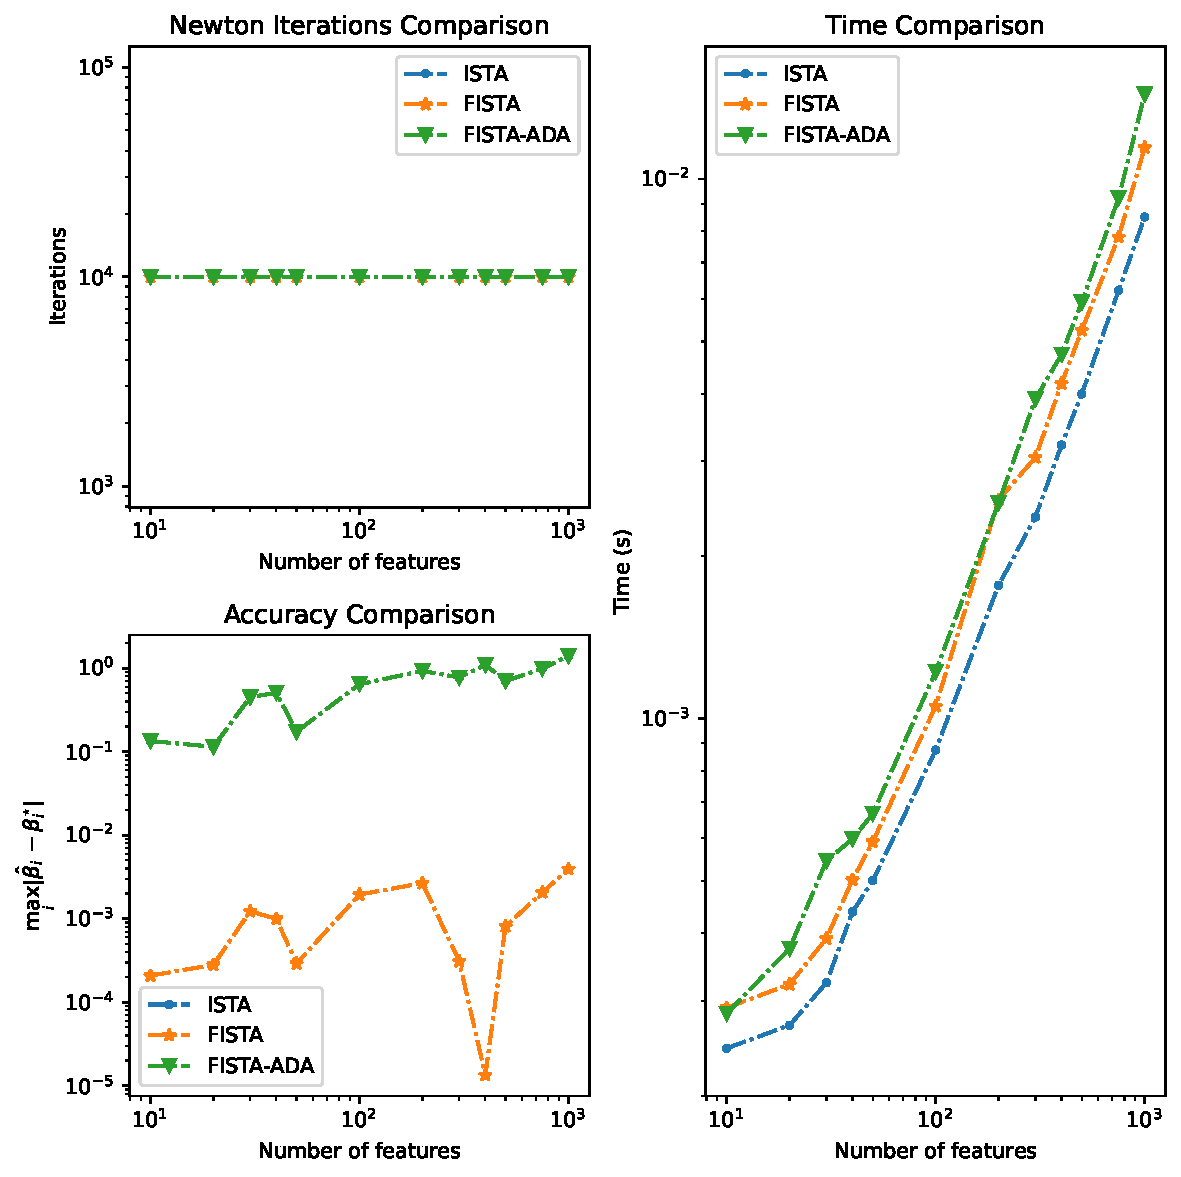
\includegraphics[width=0.5\textwidth]{figures/pgd_newton_bad_convergence.pdf}
%    \caption{Time, accuracy, and number of iterations comparison across
%    \Cref{alg:pgd:fista,alg:pgd:fista-adares,alg:pgd:ista}.
%    All methods failed to converge with max number of iterations $\num{1e4}$.
%    }
%    \label{fig:pgd:bad_convergence}
%\end{figure}
